\documentclass[10pt,a4paper]{article}
\usepackage[margin=2.1cm]{geometry}
\usepackage{amsmath,amssymb,bm}
\usepackage{graphicx,booktabs,xcolor,enumitem,hyperref}
\hypersetup{colorlinks,linkcolor=blue!50!black,urlcolor=blue!50!black}
\newcommand{\ka}{\kappa_1}
\newcommand{\kc}{\kappa_2}
\newcommand{\kb}{\bar\kappa}
\newcommand{\note}[1]{\par\smallskip\noindent\colorbox{gray!12}{\parbox{\dimexpr\linewidth-2\fboxsep}{\small #1}}\par\smallskip}
\newcommand{\evd}[1]{\textsf{\small[#1]}}
\newcommand{\simple}[1]{\par\noindent\textbf{In simple words:} #1\par\smallskip}
\title{TOP-Q --- Day 3 worked notes\\[2pt]\large A fair topological-vs-trivial comparison, disorder models, and the real hardware}
\author{PH 5110 term paper --- Kotapati Kishore (EE26E016)}
\date{25 October 2026}
\begin{document}\sloppy\maketitle

\note{Labels: \evd{Derived} \evd{Verified-by-test} \evd{Simulated} \evd{Literature} \evd{Hypothesis}.
Units: all $b$, $\kappa$, $\delta\beta$ in units of $\kc$; baseline $r=\ka/\kc=1/3$ (decision D2); $M=41$ guides.
\textbf{Schedule:} Day 3 was planned for 24 Oct and is done on 25 Oct; the one-day slip is absorbed by the Day 7 buffer.}

\tableofcontents

%=====================================================================
\section{Why the comparison must be designed, not picked}
%=====================================================================
The research question compares a \emph{topological} mode with an \emph{ordinary} one. But an ordinary defect can be made as tightly or as loosely confined as we like. If we pick a loosely confined one, it will look fragile; if we pick a tightly confined one, it will look robust. Either way the ``result'' would be decided by our choice, not by physics (risk R7). So we fix \textbf{one rule for matching} before running any Monte Carlo, and write down why.

%=====================================================================
\section{Array T: the topological interface (from the literature)}
%=====================================================================
\textbf{Geometry.} Following Blanco-Redondo \emph{et al.}\ (2016) \evd{Literature}, the topological structure is a \textbf{``long-long'' domain wall}: the centre guide has a \emph{wide} gap (weak coupling $\ka$) on \emph{both} sides; moving outward the couplings alternate $\kc,\ka,\kc,\dots$ (Fig.~\ref{fig:hw}a). It is two SSH chains glued back to back, mirror images of each other.

\textbf{Mode} \evd{Derived}. Exactly as on Day 2 but in both directions: on the centre's sublattice the amplitude is multiplied by $-r$ per cell; on the other sublattice it is zero:
\[
\psi_{2j}=\psi_0(-r)^{|j|},\qquad \psi_{2j+1}=0,\qquad b_T=0\ \text{exactly}.
\]
The array has an odd number of guides and only A--B couplings, so the Day-2 counting argument guarantees this zero mode for any coupling values. Numerically $|b_T|=2\times10^{-16}$ and the eigenvector matches the formula to $10^{-12}$ \evd{Verified-by-test}.

\simple{light put in the centre guide sits there because both its neighbours are only weakly attached. The little light that leaks out skips every second guide.}

%=====================================================================
\section{A surprise: the ``short-short'' wall is not trivial in our model}
%=====================================================================
Blanco-Redondo \emph{et al.}\ also built a ``short-short'' structure (narrow gaps next to the centre) and reported \emph{trivial} defect modes there, which they attributed to the three closely spaced guides forming a region of higher effective index \evd{Literature}.

We built the same wall with couplings only. Result \evd{Simulated; Verified-by-test}: it is chiral-symmetric and has three near-zero modes --- one on the two guides \emph{next to} the centre (the centre guide itself stays dark, power $<10^{-9}$) and two at the array ends. In a nearest-neighbour coupling model, a short-short wall is just the \emph{other} kind of SSH domain wall, which also carries a mid-gap state.

\textbf{What this means.} The trivial behaviour they saw comes from physics \emph{not in our model}: the extra effective index of closely packed guides is an \textbf{on-site} effect (the same kind as Limitation L1). So the paper's short-short structure cannot serve as our trivial reference unless we add on-site terms whose size we do not know. \textbf{Decision D5:} our trivial reference is an explicit, controlled on-site defect (array D below).

\note{\textbf{Viva point.} ``Topological vs trivial'' is a property of a \emph{model}. The same physical structure can look different in a coupling-only model and in the real device. Say which model you mean.}

%=====================================================================
\section{Array D: a conventional defect with matched confinement}
%=====================================================================
\textbf{Geometry.} Same number of guides, every coupling equal to the mean $\kb=(\ka+\kc)/2=2/3$, and the centre guide's propagation constant raised by $\Delta$ (a slightly wider guide, Fig.~\ref{fig:hw}b).

\subsection{Bound mode \evd{Derived}}
Try $\psi_n=q^{|n|}$ with $0<q<1$. Away from the centre, $b\,\psi_n=\kb(\psi_{n-1}+\psi_{n+1})$ gives $b=\kb(q+1/q)$. At the centre, $b\,\psi_0=\Delta\psi_0+2\kb q$ gives $b=\Delta+2\kb q$. Equating:
\[
\kb\Big(\frac1q-q\Big)=\Delta\ \Rightarrow\ q=\frac{\sqrt{\Delta^2+4\kb^2}-\Delta}{2\kb},\qquad b_D=\sqrt{\Delta^2+4\kb^2}.
\]
The mode exists for any $\Delta>0$ and sits \emph{above} the band of the uniform array ($|b|\le2\kb$). Nothing pins $b_D$: it moves whenever $\Delta$ or $\kb$ moves.

\subsection{The matching rule: equal IPR \evd{Derived}}
Inverse participation ratio $\mathrm{IPR}=\sum|\psi_n|^4$ (normalised mode): 1 = all light in one guide.
For power $p_n\propto q^{2|n|}$:
\[
\mathrm{IPR}(q)=\frac{(1+q^4)(1-q^2)}{(1+q^2)^3}.
\]
The T mode has \emph{the same formula with $q\to r$} (its zeros do not change the sums). So equal IPR $\Leftrightarrow q=r$, giving
\[
\boxed{\Delta=\kb\Big(\frac1r-r\Big)=\tfrac{16}{9}\kc,\qquad b_D=\tfrac{20}{9}\kc,\qquad \mathrm{IPR}_T=\mathrm{IPR}_D=0.656.}
\]
\textbf{Why IPR, and not something else?} Section 6 shows that, to first order, an on-site error spreads $b$ by $\sigma_\beta\sqrt{\mathrm{IPR}}$ for \emph{any} mode. Matching IPR therefore makes T and D \textbf{equally exposed to on-site disorder by construction}. Any difference we then see under coupling disorder is due to the structure (topology), not to confinement.
\textbf{Honest limitations of D} (record as L6): D sits in a gapless uniform array, T in a gapped one; D's mode is above the band, T's is mid-gap; IPR matching makes D decay per \emph{guide} while T decays per \emph{two guides}. A sensitivity check with another matching rule (equal decay length per guide) is an optional Day-4 item.

\begin{figure}[t]\centering
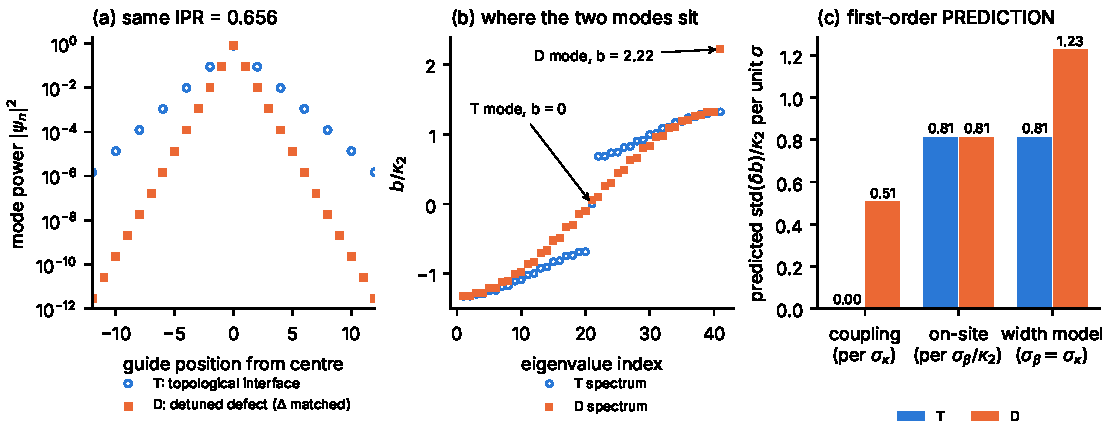
\includegraphics[width=\linewidth]{../../figures/fig_design.pdf}
\caption{Generated by \texttt{scripts/day3\_design.py} from \texttt{data/day3\_design.npz}. (a) Mode power of T and D with equal IPR. (b) Spectra: T mode at $b=0$ in the gap; D mode above the band at $b=2.22\kc$. (c) First-order \textbf{predictions} (not Monte Carlo) of the spread of $b$ per unit disorder strength.}
\label{fig:design}
\end{figure}

%=====================================================================
\section{Disorder models (what each one means physically)}
%=====================================================================
\subsection{Coupling disorder: log-normal, and why \evd{Derived}}
On Day 1: $\kappa=\kappa_0e^{-\gamma g}$. If the gap error $\delta g$ is Gaussian, then $\ln\kappa$ changes by $-\gamma\,\delta g$, which is Gaussian. So $\kappa\to\kappa\,e^{\sigma_\kappa g}$, $g\sim\mathcal N(0,1)$, $\sigma_\kappa=\gamma\sigma_g$, is \emph{exactly} what a Gaussian gap error produces, and $\kappa$ can never go negative. Keeps chiral symmetry. \evd{Verified-by-test: positive, $\langle\ln\rangle=0$, std $=\sigma_\kappa$}

\subsection{On-site disorder}
$\delta\beta_n=\sigma_\beta g_n$: each guide's propagation constant is off by a random amount (width or height error). Breaks chiral symmetry.

\subsection{Width model: the realistic, mixed case}
One width error $\delta w_n$ per guide changes \emph{two} things at once:
\[
\delta\beta_n=\sigma_\beta\,\delta w_n,\qquad \kappa_{n,n+1}\to\kappa_{n,n+1}\exp\!\Big[\sigma_\kappa\frac{\delta w_n+\delta w_{n+1}}{2}\Big].
\]
Sign logic: if the guide centres are fixed by the mask, a wider guide leaves a narrower gap, so the coupling grows. Neglected: the direct change of $\kappa$ with how tightly a wider mode is confined (\textbf{L5}). The ratio $\sigma_\beta/\sigma_\kappa$ depends on the waveguide and \textbf{is not known yet} (needs a mode solver); Day 4 scans it rather than guessing it. \evd{Verified-by-test: correlation between a guide's $\delta\beta$ and its couplings $>0.6$}

\subsection{Global shift}
One common offset on all guides (wafer-scale thickness error). Breaks chiral symmetry but adds the same phase to everything, so it cancels in relative-phase measurements (Day 2, question 2).

\subsection{Reproducible random numbers}
Each Monte Carlo sample $s$ gets its own generator from \texttt{SeedSequence([seed, s])}. The same seed and sample number always give the same numbers, and the result does not depend on the order in which samples are run \evd{Verified-by-test}.

%=====================================================================
\section{First-order predictions (to be tested on Day 4)}
%=====================================================================
For a small change $\delta H$, the eigenvalue moves by $\delta b\approx\langle\psi|\delta H|\psi\rangle$ (first-order perturbation theory) \evd{Derived; Verified-by-test against exact diagonalisation, error $<10^{-10}$}:
\[
\delta b\approx\sum_n\psi_n^2\,\delta\beta_n+2\sum_n\psi_n\psi_{n+1}\,\delta\kappa_n .
\]
\begin{itemize}[itemsep=1pt]
\item \textbf{T under coupling disorder:} $\psi_n\psi_{n+1}=0$ for every bond (one sublattice is empty), so the first-order shift is \emph{zero}. (Day 2 showed it is zero to \emph{all} orders.)
\item \textbf{On-site disorder, any mode:} $\mathrm{std}(\delta b)=\sigma_\beta\sqrt{\sum\psi_n^4}=\sigma_\beta\sqrt{\mathrm{IPR}}$. Equal for T and D by design.
\item \textbf{Width model:} T feels only the on-site part; D feels both, and they add because they are correlated.
\end{itemize}

\begin{tabular}{@{}lccc@{}}\toprule
Predicted std$(\delta b)/\kc$ per unit $\sigma$ & coupling ($\sigma_\kappa$) & on-site ($\sigma_\beta$) & width ($\sigma_\beta=\sigma_\kappa$)\\\midrule
T (topological interface) & $0.00$ & $0.81$ & $0.81$\\
D (matched defect) & $0.51$ & $0.81$ & $1.23$\\\bottomrule
\end{tabular}\par\smallskip

\textbf{Hypotheses for Day 4.} \textbf{H3}: under coupling disorder T stays at $b=0$ while D spreads as $0.51\sigma_\kappa$ for small $\sigma$. \textbf{H4}: under on-site disorder T and D spread \emph{equally} ($0.81\sigma_\beta$): topology gives \emph{no} protection here. \textbf{H5}: under the width model T is better than D only by removing the coupling part; how much better depends on the unknown ratio $\sigma_\beta/\sigma_\kappa$.
\note{\textbf{Big picture.} If H4 holds, the first honest conclusion of TOP-Q is already visible: topological protection removes \emph{one} error channel (coupling errors) and does nothing for another (propagation-constant errors). Whether real fabrication errors are mostly one or the other decides how useful the protection is.}

%=====================================================================
\section{The real hardware}
%=====================================================================
\textbf{What is ours and what is not.} We have \textbf{no} fabricated chip, laser or camera. Every number in TOP-Q is a simulation. The hardware below is the \emph{published} platform that our model describes.

\begin{figure}[!htbp]\centering
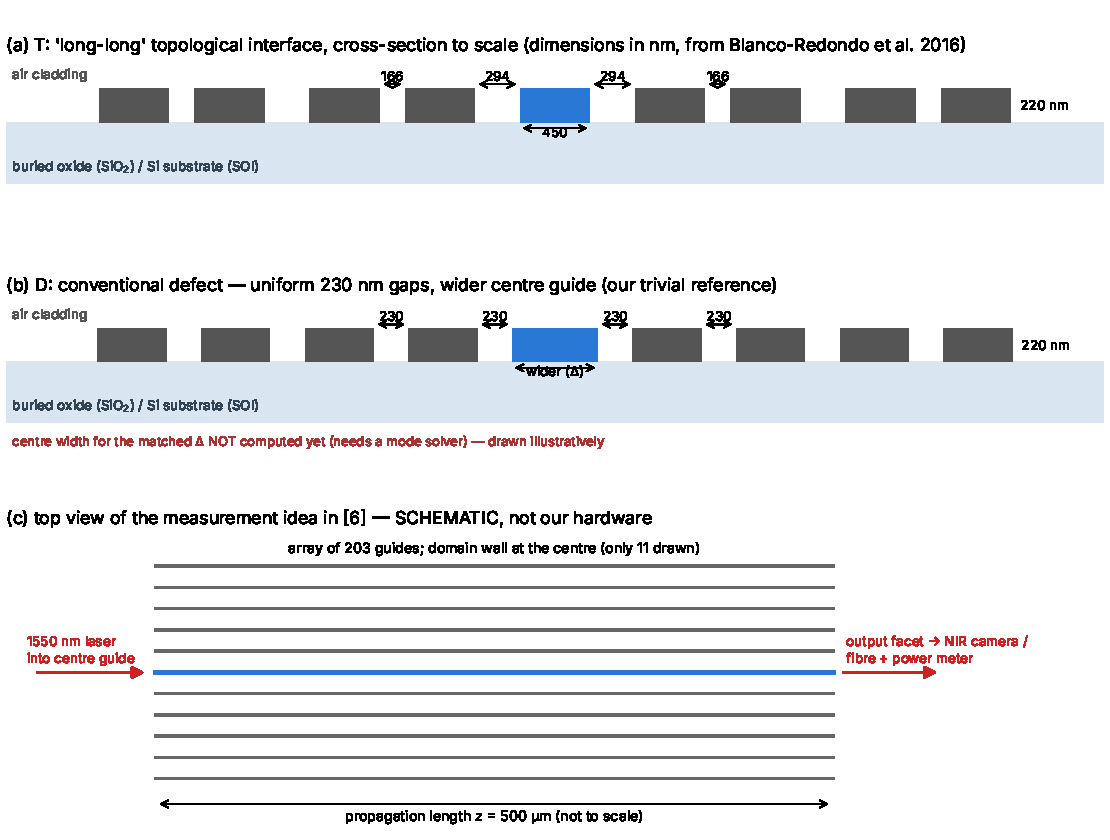
\includegraphics[width=0.92\linewidth]{../../figures/fig_hardware_schematic.pdf}
\caption{\textbf{Schematic drawn by us} (not a photograph). Cross-sections to scale with dimensions from Blanco-Redondo \emph{et al.}\ (2016): Si waveguides $450\times220$~nm on silicon-on-insulator, air cladding, 203 guides, 500~$\mu$m long, $\lambda=1550$~nm; long-long gaps 294/166~nm. (b) Our trivial reference D; the wider centre width is illustrative because the width that gives the matched $\Delta$ has not been computed. (c) Measurement idea: light into the centre guide, output imaged with a near-infrared camera and measured with a fibre and power meter.}
\label{fig:hw}
\end{figure}

\subsection{How the real device works (step by step)}
\begin{enumerate}[itemsep=1pt]
\item \textbf{Chip.} A silicon-on-insulator wafer: a 220~nm silicon layer on a buried oxide layer on a silicon substrate. Deep-UV lithography (at IMEC in the paper) and etching leave silicon strips 450~nm wide --- these are the waveguides. Air above acts as cladding.
\item \textbf{The design is only in the gaps.} All guides are identical; the SSH pattern is written by alternating the gaps (166 and 294~nm). This is why gap errors $\to$ coupling disorder, and width errors $\to$ both (Section 5.3).
\item \textbf{Input.} A 1550~nm laser is coupled into the centre guide.
\item \textbf{Propagation.} 500~$\mu$m of propagation; the paper notes this should be at least about 10 coupling lengths.
\item \textbf{Output.} The light leaving the end of the array is imaged on a near-infrared camera, and the power in each guide is measured with a fibre connected to a power meter.
\item \textbf{Result reported.} The long-long (topological) structure kept light in the centre guide with the same output over an 8~nm wavelength range; the short-short structure showed beating between two modes that changed with length and wavelength \evd{Literature}.
\end{enumerate}

\subsection{Published hardware images to look at and cite}
Real photographs and SEM images are owned by their publishers, and my workspace cannot download them, so they are \textbf{not} pasted into these notes. They were shown in our chat, and you can find them here:
\begin{tabular}{@{}p{0.42\linewidth}p{0.5\linewidth}@{}}\toprule
Source & What to look for\\\midrule
Blanco-Redondo \emph{et al.}, PRL \textbf{116}, 163901 (2016) & device images of the silicon arrays and measured output patterns (the platform we model)\\
Review ``Topological silicon photonics'', \emph{Advanced Photonics Research} (2021) --- \emph{verify authors and DOI} & SEM images of many silicon topological devices\\
Review ``Integrated topological photonics in one dimension'' (Taylor \& Francis) --- \emph{verify authors, journal and DOI} & 1-D SSH chips, fabrication and measurement setups\\
Femtosecond-laser-written waveguides in fused silica (several groups) & a second real SSH platform: waveguides written inside glass, with fluorescence imaging of light inside the array\\\bottomrule
\end{tabular}\par\smallskip\noindent\textbf{Rule for the paper:} any real photo must say ``Reproduced from [ref]'' and should come from an open-access (CC-BY) source or have permission. Never caption it as our own device.

%=====================================================================
\section{Code and tests}
%=====================================================================
New: \texttt{topq/arrays.py} (T, D and SS arrays, matched $\Delta$, analytic modes), \texttt{topq/disorder.py} (coupling, on-site, width and global disorder; reproducible generators; first-order predictions). \texttt{tests/test\_arrays\_disorder.py}: 16 new tests, including a 3000-sample Monte Carlo check of the width-model prediction (agreement within 5\%). Whole suite: \textbf{70 passed}.

\section{Self-test (answer without notes)}
\begin{enumerate}[itemsep=1pt]
\item Why would picking an arbitrary trivial defect make the comparison meaningless?
\item Derive $b_D=\sqrt{\Delta^2+4\kb^2}$ in three lines.
\item Why does matching IPR make T and D equally sensitive to on-site errors?
\item Why is a Gaussian gap error the same thing as log-normal coupling disorder?
\item In the width model, why does a wider guide \emph{increase} its neighbours' couplings?
\item The paper calls the short-short modes trivial, but our model finds a mid-gap state. Who is wrong?
\end{enumerate}
\end{document}
